\documentclass[11pt]{article}

% Load packages
\usepackage{amsmath, amsfonts} % for math
\usepackage{graphicx} % for figures
\usepackage[margin=1in]{geometry} % to set margins
\usepackage{tcolorbox} % to create nice boxes
\tcbuselibrary{skins,breakable} % extra libraries for the nice boxes
\usepackage{listings}
\usepackage{enumerate}
\usepackage{empheq}

% Define a custom box for the solutions. Don't change this!
\newtcolorbox[]{solution}
    {colframe=red!20, 
        colback=white, 
        sharp corners,
        title=Solution,
        enhanced,
        coltitle=black,
        fonttitle=\bfseries,
        attach boxed title to top left={yshift*=-\tcboxedtitleheight/2, xshift=3mm},
        boxed title style={sharp corners, colback=red!20}
        }

\usepackage{boondox-calo}

\newcommand{\lr}[1]{\left(#1\right)}

\usepackage{hyperref}
\hypersetup{
    colorlinks=true,
    linkcolor=blue,
    filecolor=magenta,      
    urlcolor=cyan
}

% MSE Set graphics path
\graphicspath{{figs/}}

% MSE Terminal environment for screenshots
\lstdefinestyle{Terminal}
{
    basicstyle=\fontsize{9}{11}\color{black}\ttfamily
}

% MSE Code snippets
\lstdefinestyle{CodeSnippet}
{
    basicstyle=\fontsize{10}{12}\color{black}\ttfamily
}
% MSE Macros
\newcommand{\tty}[1]{\texttt{#1}}

% Write the document
\begin{document}

    \title{Extreme Computing: Homework 2}
    \author{Michael S. Emanuel, Jonathan Guillotte-Blouin, Yue Sun}
    \date{April 15, 2019}
    \maketitle

  \section{Problem 1:  Channel Flow with a central narrowing}
    Simulating channel flow in 2D with a narrowing is the target.

The type of flow in absence of the narrowing is the well-known Hagen-Poiseuille flow 
(and by the way, Poiseuille was a physicist and physiologist who studied blood flows 
in a systematic way).

Let's write the corresponding grid for a straight channel aligned along, say, the x axis. 

When constructing the grid and using it in the LBM context 
you should apply what you have learned about grid management. 

Let's recall that in absence of open boundaries (inlet or outlet), each fluid node should always 
be surrounded by other fluid or wall nodes to preserve mass and momentum locally (no leakage rule).

The solution should employ two different options:

    \begin{enumerate}
      \item A periodic channel (aligned with the x direction): start from a quiescent fluid and
      apply a body acceleration uniformly through the fluid until you match the Reynolds number at steady state.
      \item A non-periodic channel with inlet and outlet faces and by applying a uniform velocity 
      at inlet and outlet with plug flow profiles.
    \end{enumerate}

    Use no-slip boundary conditions at the walls and a Reynolds number of $10^{-2}$ computed from fluid velocity 
    imposed at $x=0$ (the inlet region for non-period channel) and characterstic length being $H$.

    \begin{figure}[h!]
      \centering{}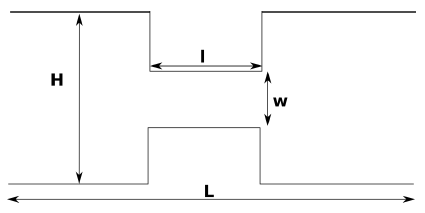
\includegraphics[scale=1.0]{narrowing.png}
      \caption{The geometry for the channel with central narrowing.}
      \label{fig:narrowing}
    \end{figure}

    
    \textbf{For a fixed set of values for the geometry 
    as in Fig. \ref{fig:narrowing}, (suggested values $L=200$, $H=60$, $l=50$, $w=30$), 
    calculate the following quantities:}
    \begin{enumerate}
      \item The pressure field
      \item The velocity field 
      \item The volume flow rate 
      \item The average and maximum velocities in the channel
    \end{enumerate}

    Repeat the simulation by varying the width of the narrowing $w$.

Our solution to this problem can be found in the folder \tty{hw2/lbm\_7}
in our team's repository for this course.  
Here is a brief overview of the components in our solution.
The files \tty{lattice.hh} declares and implments the class \tty{lattice}
(that is, it's a header-only implemenation).  
One instance of this class represents a single point on the lattice.

The driver programs \tty{lbm\_pbc} and \tty{}

    \textbf{Plot:}
    Show how the flow rate changes by varying $w$ in the range $0<w<50$

    Compare the pressure at the narrowing with the simple Bernoulli estimate for inviscid flows, stating that
    $$
    \frac{1}{2} \rho u_o^2 + p_o = \frac{1}{2} \rho u_i^2 + p_i
    $$
    where $u_o$ and $p_o$ are cross-sectional averages of velocity and pressure at $x=0$ for a periodic system 
    or at the inlet otherwise, and $u_i$ and $p_i$ are the same quantities at the center of the narrowing. 
    
    \textbf{Plot:}
    Plot the obtained pressure vs the Bernoulli estimate by varying the LBM kinematic viscosity in the range 0.05 : 0.1667.

%%% PROBLEM 2 %%%
  \section{Problem 2:  Basic CUDA and GPUs}
    \textit{This problem was submitted by Dan Willen \texttt{daniel.p.willen@gmail.com}}

    Consider the equation
    \begin{equation}\label{eq:heat}
      \frac{\partial u}{\partial t} = D \nabla^2 u,
    \end{equation}
    on the domain \(0 \leq x,y \leq \pi\), with \(u = u(x,y,t)\), \(D\) the diffusive constant, and \(\nabla^2\) the Laplace operator.
    The boundary conditions are of the homogeneous Dirichlet type:
    \begin{equation}
      u(x = 0, y) = u(x = \pi, y) = u(x, y = 0) = u(x, y = \pi) = 0,
    \end{equation}
    and the initial condition is
    \begin{equation}
      u(x,y, t = 0) = \sin(x) \sin(y).
    \end{equation}
    The solution to this equation is
    \begin{equation}
      u(x,y,t) = \sin(x) \sin(y) \exp{(-2Dt)}
    \end{equation}
    
    Using a second-order central difference in space and first order forward difference in time, the discretization of \eqref{eq:heat} is
    \begin{equation}
      u_{i,j}^{\left(n+1\right)} = u_{i,j}^{\left(n\right)} + \frac{D \Delta t}{\Delta x^2} 
        \left[u_{i+1, j}^{\left(n\right)} +
              u_{i-1, j}^{\left(n\right)} +
              u_{i, j+1}^{\left(n\right)} +
              u_{i, j-1}^{\left(n\right)} -
              4u_{i, j}^{\left(n\right)} \right],
    \end{equation}
    where \(u_{i,j}^{\left(n\right)}\) is the value of \(u\) at the \(n^{th}\) time step at grid point \((i,j)\), \(\Delta t = \Delta x^2 / 4D\) is the time step size, and \(\Delta x\) is the grid spacing in the \(x\) and \(y\) directions.
    
    \vspace{5mm}
    
    \begin{enumerate}
      \item Using Cuda, solve the discretized equations up to a time \(t = \pi^2/D\) using the Jacobi method.
        A skeleton code is provided to assist you, with comments in the locations you should make changes.
        \begin{enumerate}[Step I --]
          \item Declare, allocate, and initialize memory for the field variable \texttt{u} on the CPU.
            You should allocate enough memory for the grid, which has size \(nx \times ny\) and initialize \texttt{u} to the initial condition.
            Make sure you free the memory at the end of the program.
          \item Declare and allocate the GPU memory for \texttt{\_u}, \texttt{\_u\_new}\, and \texttt{\_error}.
            Copy the CPU memory to the GPU; the other two arrays have been initialized to zero for you.
            Make sure you free the memory at the end of the program.
          \item Set up the kernel execution configuration for the GPU kernel based on the input domain size and the maximum threads per dimension,
            which is set at the top of the file as a \texttt{\#define}.
            You will need to determine the number of threads per block and the number of blocks in each direction, as well as set up the \texttt{dim3} variables.
          \item Write a GPU kernel that advances to the next timestep using the Jacobi method.
            This should be done in parallel, not in serial.
          \item Write a GPU kernel that calculates the error between the numerical and analytic solutions at each point.
            Be careful to compare solutions at the correct timestep -- \texttt{\_u\_new} is at \(t = (n+1) \Delta t\) and \texttt{\_u} is at \(t = n \Delta t\).
            Using this result, a parallel reduction using the Thrust parallel algorithms library has been provided to calculate the total error in order to find the average percent error at each grid point.
          \item At the end of the loop, copy the data back to the CPU.
        \end{enumerate}
    \end{enumerate}
    
    Your program should take as an input the number of grid cells on one side of the domain.
    This has been set up for you such that the program can be run from the command line like: 
    \vspace{3mm}\\ \texttt{./jacobi\_solver.cu n} \vspace{3mm}\\
    where \(nx = ny = \) \texttt{n} is the size of one side of the square domain.
    The program should output the percent difference between your result and the analytic solution, averaged over all of the grid nodes:
    \begin{equation}
      \epsilon = \frac{1}{n_x n_y} \sum_{i=1}^{n_x} \sum_{j=1}^{n_y} \frac{u_{i,j}^{\left(n\right)} -
U_{i,j}^{\left(n\right)}}{U_{i,j}^{\left(n\right)}},
    \end{equation}
    where \(U\) is the analytic solution.
    
    If you have time, discuss the following:
    \begin{itemize}
      \item How does the error change as you increase the resolution? Does this behavior make sense?
      \item How does the runtime scale with the resolution? You can get a rough estimate by using the bash command \texttt{time} when executing your program, like:
    \vspace{3mm}\\ \texttt{./jacobi\_solver.cu n} \vspace{3mm}\\ and using the result for \texttt{real}. \\
      \item How does the runtime change as you change the kernel execution configuration?
        e.g., play around the \texttt{MAX\_THREADS\_DIM} parameter as well as different schemes for setting up the thread blocks.
      \item Use shared memory in the Jacobi kernel
    \end{itemize}


\end{document}

